%==============================================================================
%  Homework template  --  999 Controls
%
%  To reuse for the next assignment:
%    1. copy this folder,  2. edit the METADATA block below,
%    3. edit the SOLUTIONS section,  4. run  `make`.
%
%  Build:  make          (regenerates code output, then builds main.pdf)
%          make clean    (removes build artifacts)
%==============================================================================
\documentclass[11pt,letterpaper]{article}

%------------------------------- METADATA -------------------------------------
\newcommand{\hwcourse}{EE 999 --- Introduction to Control Systems}
\newcommand{\hwcourseshort}{EE 999}  % running head, keep it short
\newcommand{\hwtitle}{Homework 10}
\newcommand{\hwauthor}{Patrick Gordon}
\newcommand{\hwdate}{\today}
\newcommand{\hwdue}{Due Wednesday, December 2, 2026}
%------------------------------------------------------------------------------

\usepackage[T1]{fontenc}
\usepackage[utf8]{inputenc}
\usepackage{textcomp}
\usepackage[letterpaper,margin=1in,headheight=14pt]{geometry}
\usepackage{amsmath,amssymb}
\usepackage{cancel}
\usepackage{array}
\usepackage{graphicx}
\usepackage[american]{circuitikz}
\usepackage{xcolor}
\usepackage{listings}
\usepackage{fancyhdr}
\usepackage{inconsolata}
\usepackage{pdflscape}
\usepackage{float}
\usepackage[hidelinks]{hyperref}

%--- page furniture -----------------------------------------------------------
\pagestyle{fancy}
\fancyhf{}
\lhead{\hwauthor}
\chead{\hwtitle}
\rhead{\hwcourseshort}
\cfoot{\thepage}

%--- listing styles -----------------------------------------------------------
\definecolor{codebg}{HTML}{F7F7F4}
\definecolor{outbg}{HTML}{FCFCFC}
\definecolor{rule}{HTML}{C8C8C0}
\definecolor{kw}{HTML}{1C4FA1}
\definecolor{cmt}{HTML}{6A7A5A}
\definecolor{str}{HTML}{A0522D}

\lstdefinestyle{mcode}{
  language=Octave,
  basicstyle=\ttfamily\footnotesize,
  keywordstyle=\color{kw}\bfseries,
  commentstyle=\color{cmt}\itshape,
  stringstyle=\color{str},
  backgroundcolor=\color{codebg},
  frame=single,
  rulecolor=\color{rule},
  framesep=6pt,
  numbers=left,
  numberstyle=\ttfamily\scriptsize\color{gray},
  numbersep=8pt,
  showstringspaces=false,
  breaklines=true,
  columns=fullflexible,
  keepspaces=true,
  upquote=true,
}

\lstdefinestyle{moutput}{
  basicstyle=\ttfamily\footnotesize,
  backgroundcolor=\color{outbg},
  frame=single,
  rulecolor=\color{rule},
  framesep=6pt,
  showstringspaces=false,
  breaklines=true,
  columns=fullflexible,
  keepspaces=true,
  upquote=true,
  % MATLAB prints empty results as "0×1 empty double column vector"; listings
  % cannot read the UTF-8 multiplication sign without this mapping.
  literate={×}{{$\times$}}1,
}

%--- structure helpers --------------------------------------------------------
% \problem{1.1b}{Optional title}
\newcommand{\problem}[2]{%
  \bigskip
  \noindent{\large\bfseries Problem #1}%
  \ifx\relax#2\relax\else\ {\large --- #2}\fi
  \par\nobreak\vspace{2pt}\hrule\vspace{8pt}\nobreak
}

% \caplabel{Code}{hw_02_A.m}
\newcommand{\caplabel}[2]{%
  \par\nobreak\vspace{6pt}\nobreak
  \noindent{\small\bfseries #1}\ {\small\ttfamily \detokenize{#2}}%
  \par\nobreak\vspace{2pt}\nobreak
}

% \matlabcode{hw_02_A.m}  -- source listing pulled straight from the .m file
\newcommand{\matlabcode}[1]{%
  \caplabel{Code:}{#1}%
  \lstinputlisting[style=mcode]{#1}%
}

% \codeoutput{output/hw_02_A.txt} -- console output captured by the Makefile
\newcommand{\codeoutput}[1]{%
  \caplabel{Output:}{#1}%
  \IfFileExists{#1}{\lstinputlisting[style=moutput]{#1}}{\missing{#1}{run \texttt{make} to generate it}}%
}

% \answerfigure[width]{figures/foo.pdf}{Caption}  -- placeholder if not exported
% yet. Any format graphicx reads works: pdf, png, jpg.
% A script that plots is exported by the Makefile to figures/<script>.pdf, so
% \answerfigure{figures/hw_02_F.pdf}{...} is how a plotted answer is included.
% The optional argument is the printed width, default the full text width.
% Give a scan or screenshot a smaller one so it is not blown up past its own
% resolution:  \answerfigure[0.8\linewidth]{figures/some_scan.png}{...}
\newcommand{\answerfigure}[3][\linewidth]{%
  \begin{figure}[H]
    \centering
    \IfFileExists{#2}{\includegraphics[width=#1]{#2}}{\missing{#2}{export it, see README}}
    \caption{#3}
  \end{figure}%
}

% \splane{G_1(s)}  -- an empty s-plane grid to sketch poles (x) and zeros (o)
% on by hand. One unit per square, Re from -10 to 3 and Im from -4 to 4.
% \splane[5]{G_2(s)} instead centres the origin, both axes running -5 to 5.
\newcommand{\splane}[2][]{%
  \ifx\relax#1\relax
    \def\spxmin{-10}\def\spxmax{3}\def\spymax{4}\def\spxlabels{-10,-8,...,2}\def\spylabels{-4,-2,2,4}\def\spscale{1}%
  \else
    \def\spxmin{-#1}\def\spxmax{#1}\def\spymax{#1}\def\spxlabels{-#1,...,-1,1,2,...,#1}\def\spylabels{-#1,...,-1,1,2,...,#1}\def\spscale{0.85}%
  \fi
  \begin{figure}[H]
    \centering
    \begin{tikzpicture}[scale=\spscale]
      \draw[gray!30, thin] (\spxmin,-\spymax) grid (\spxmax,\spymax);
      \draw[->, thick] (\spxmin-0.3,0) -- (\spxmax+0.4,0) node[right] {$\mathrm{Re}$};
      \draw[->, thick] (0,-\spymax-0.3) -- (0,\spymax+0.4) node[above] {$\mathrm{Im}$};
      \foreach \x in \spxlabels
        \node[below, font=\scriptsize, fill=white, inner sep=1pt] at (\x,-0.05) {$\x$};
      \foreach \y in \spylabels
        \node[left, font=\scriptsize, fill=white, inner sep=1pt] at (-0.05,\y) {$\y j$};
    \end{tikzpicture}
    \caption{Pole-zero sketch of $#2$.}
  \end{figure}%
}

% \splanewindow{xmin}{xmax}{ymax}{xstep}{ystep}{scale}{Caption}  -- \splane
% with the window chosen per problem, for poles that fall outside the default.
% Re runs xmin..xmax, Im runs -ymax..ymax, axis labels every xstep / ystep, and
% a fine half-unit grid under the unit grid. scale is cm per unit, and the full
% caption is given since the window is usually showing something specific.
%   \splanewindow{-7}{1}{12}{1}{2}{0.6}{Closed-loop poles as $k_d$ varies.}
\newcommand{\splanewindow}[7]{%
  \begin{figure}[H]
    \centering
    \begin{tikzpicture}[scale=#6]
      \draw[gray!15, very thin, step=0.5] (#1,-#3) grid (#2,#3);
      \draw[gray!40, thin] (#1,-#3) grid (#2,#3);
      \draw[->, thick] (#1-0.3,0) -- (#2+0.4,0) node[right] {$\mathrm{Re}$};
      \draw[->, thick] (0,-#3-0.3) -- (0,#3+0.4) node[above] {$\mathrm{Im}$};
      \pgfmathtruncatemacro{\spxa}{#1}\pgfmathtruncatemacro{\spxb}{#1+#4}%
      \foreach \x in {\spxa,\spxb,...,#2}
        {\ifnum\x=0\else\node[below, font=\scriptsize, fill=white, inner sep=1pt] at (\x,-0.05) {$\x$};\fi}
      \pgfmathtruncatemacro{\spya}{-#3}\pgfmathtruncatemacro{\spyb}{-#3+#5}%
      \foreach \y in {\spya,\spyb,...,#3}
        {\ifnum\y=0\else\node[left, font=\scriptsize, fill=white, inner sep=1pt] at (-0.05,\y) {$\y j$};\fi}
    \end{tikzpicture}
    \caption{#7}
  \end{figure}%
}

%--- tables -------------------------------------------------------------------
% Centred paragraph column, so a description column wraps instead of running
% off the page:  \begin{tabular}{|c|P{0.5\linewidth}|}
\newcolumntype{P}[1]{>{\centering\arraybackslash}p{#1}}

% \begin{symboltable}{Signal}{Caption}  -- the symbol / units / description
% table used to define the variables of a problem. The first argument is the
% heading of the left column (Signal, Parameter, State, ...); leave the second
% empty for no caption.
%
%   \begin{symboltable}{Signal}{}
%     \sym{x(t)}{m}{Position of tire center}
%     \sym{r(t)}{m}{Road height (depends on $v_{car}(t)$)}
%   \end{symboltable}
%
% \sym puts its first argument in math mode and brackets the units, so write
% \sym{x(t)}{m}{...}, not \sym{$x(t)$}{[m]}{...}. Anything already math -- a
% subscript, a fraction -- goes in the description as usual: $\frac{1}{4}$.
%
% The optional argument is the width of the description column, for a table
% whose descriptions are much longer or much shorter than average:
%   \begin{symboltable}[0.35\linewidth]{Parameter}{}
\newcommand{\sym}[3]{$#1$ & [#2] & #3 \\ \hline}
\newenvironment{symboltable}[3][0.45\linewidth]{%
  \def\symtabcap{#3}%
  \begin{table}[H]
  \centering
  \renewcommand{\arraystretch}{1.4}
  \begin{tabular}{|c|c|P{#1}|}
  \hline
  #2 & Units & Description \\ \hline\hline
}{%
  \end{tabular}
  \ifx\symtabcap\empty\else\caption{\symtabcap}\fi
  \end{table}%
}

% \begin{answertable}{|c|c|c|}{Caption} -- any other table. Same placement and
% captioning as \answerfigure, but you write the rows yourself:
%
%   \begin{answertable}{|c|P{0.5\linewidth}|}{Pole locations.}
%     \hline
%     Pole & Behaviour \\ \hline\hline
%     $s=-2$ & decays in half a second \\ \hline
%   \end{answertable}
\newenvironment{answertable}[2]{%
  \def\anstabcap{#2}%
  \begin{table}[H]
  \centering
  \renewcommand{\arraystretch}{1.4}
  \begin{tabular}{#1}
}{%
  \end{tabular}
  \ifx\anstabcap\empty\else\caption{\anstabcap}\fi
  \end{table}%
}

% \begin{termtable}{4}{Caption} -- collect like powers of $s$ when multiplying
% out a characteristic polynomial (or any other expansion). The argument is the
% highest power; the columns and the $s^4 \dots s^0$ header are generated from
% it, so changing the degree is a one-character edit. Leave the second argument
% empty for no caption.
%
% Cells are already in math mode: write m_1m_2, not $m_1m_2$. One row per factor
% you multiplied out, one column per power; leave a cell empty where that factor
% contributes nothing to that power. Rows end with \\, like any tabular.
%
%   \begin{termtable}{4}{Terms of the characteristic polynomial.}
%     m_1m_2 & m_1b & m_1k_s       & bk_s       & k_s(k_s+k_w) \\
%            & m_2b & m_2(k_s+k_w) & b(k_s+k_w) &              \\
%            &      & -b^2         & -bk_s      & -k_s^2
%   \end{termtable}
%
% M is a centred column that is always in math mode. It uses \( \) rather than
% $ $ so that an empty cell stays empty -- a bare $$ would start display math.
\newcolumntype{M}{>{\(}c<{\)}}
\makeatletter
\newcount\tt@i
\newcommand{\tt@cols}{}
\newcommand{\tt@head}{}
\newcommand{\tt@build}[1]{%
  \def\tt@cols{}\def\tt@head{}%
  \tt@i=#1\relax
  \@whilenum\tt@i>\m@ne\do{%
    \edef\tt@cols{\tt@cols M}%
    \ifx\tt@head\@empty
      \edef\tt@head{s^{\the\tt@i}}%
    \else
      \edef\tt@head{\tt@head & s^{\the\tt@i}}%
    \fi
    \advance\tt@i\m@ne
  }%
}
\newenvironment{termtable}[2]{%
  \def\tt@cap{#2}%
  \tt@build{#1}%
  \begin{table}[H]%
  \centering
  \setlength{\tabcolsep}{12pt}%
  \renewcommand{\arraystretch}{1.3}%
  \edef\@tempa{\noexpand\begin{tabular}{\tt@cols}}\@tempa
  \tt@head \\ \hline
}{%
  \end{tabular}
  \ifx\tt@cap\@empty\else\caption{\tt@cap}\fi
  \end{table}%
}
\makeatother

% wideproblem environment -- a problem on its own landscape page, centred.
% Use for diagrams much wider than they are tall, where a portrait page would
% shrink the labels below readable size:
%   \begin{wideproblem}{1.1b}{Title}
%     \answerfigure{figures/x.pdf}{Caption}
%   \end{wideproblem}
\newenvironment{wideproblem}[2]{%
  \begin{landscape}%
    \problem{#1}{#2}%
    \vspace*{\fill}%
}{%
    \vspace*{\fill}%
  \end{landscape}%
}

% \prompt{What special property does b*d have?} -- restate the question
\newcommand{\prompt}[1]{%
  \noindent\textit{#1}\par\vspace{6pt}%
}

% \subpart{D.1} -- bold label for a numbered sub-part of a problem
\newcommand{\subpart}[1]{%
  \noindent\textbf{#1}\par\vspace{4pt}%
}

% \answer{...}  -- written answer. Leave the body empty for a visible
% placeholder box; fill it in and the box is replaced by the prose.
\newcommand{\answer}[1]{%
  \ifx\relax#1\relax\todo{write the answer here}\else#1\fi
  \par\vspace{4pt}%
}

\newcommand{\todo}[1]{%
  \fbox{\parbox{0.9\linewidth}{\centering\vspace{10pt}\rmfamily\itshape\small
    #1\vspace{10pt}}}%
}

\newcommand{\missing}[2]{%
  \fbox{\parbox{0.9\linewidth}{\centering\vspace{10pt}\ttfamily\small
    missing: \detokenize{#1}\\[4pt]\rmfamily\itshape #2\vspace{10pt}}}%
}


%==============================================================================
\begin{document}

\begin{center}
  {\LARGE\bfseries \hwtitle}\\[4pt]
  {\large \hwcourse}\\[8pt]
  {\hwauthor} \quad\textbullet\quad {\hwdate}\\[4pt]
  {\small\itshape \hwdue}
\end{center}
\vspace{6pt}\hrule

%------------------------------------------------------------------------------
%  SOLUTIONS
%------------------------------------------------------------------------------


\clearpage
\problem{1}{PD and PI Motor Control}
\answerfigure{figures/fig_hw10_1.png}{Block diagram with controller and plant.\label{fig:hw10-1}}
\begin{answertable}{|c|c|c|}{Controller and plant combinations.\label{tab:hw10-cases}}
  \hline
  Case & $G_c(s)$ & $G_p(s)$ \\ \hline\hline
  A & $k_d s + k_p$         & $\dfrac{k_t}{Js + b}$     \\[8pt] \hline
  B & $\dfrac{k_p s + k_i}{s}$ & $\dfrac{k_t}{Js + b}$     \\[8pt] \hline
  C & $k_d s + k_p$         & $\dfrac{k_t}{Js^2 + bs}$  \\[8pt] \hline
  D & $\dfrac{k_p s + k_i}{s}$ & $\dfrac{k_t}{Js^2 + bs}$  \\[8pt] \hline
\end{answertable}

\problem{1.A}{System Type}
\prompt{With the block diagram of Figure~\ref{fig:hw10-1}, determine the system type for each combination of $G_c(s)$ and $G_p(s)$, A to D. The Bode standard form is
\[
  G(s) = K_{Bode}\,\frac{1}{s^{n_0}}\,\frac{b_m s^m + \dots + b_1 s + 1}{a_n s^n + \dots + a_1 s + 1},
\]
where $n_0$ is the number of poles at the origin (and gives the system type).}
\subpart{A}
\answer{
\begin{align}
  G_A(s) &= (k_d s + k_p)\left(\frac{k_t}{Js + b}\right) \label{eq:1A-A-prod} \\
  G_A(s) &= \frac{k_d k_t\,s + k_p k_t}{Js + b} \label{eq:1A-A-mult}
\end{align}
Since $n_0 = 0$, the system is Type 0.
}
\subpart{B}
\answer{
\begin{align}
  G_B(s) &= \left(\frac{k_p s + k_i}{s}\right)\left(\frac{k_t}{Js + b}\right) \label{eq:1A-B-prod} \\
  G_B(s) &= \frac{k_p k_t\,s + k_i k_t}{s\,(Js + b)} \label{eq:1A-B-mult}
\end{align}
Since $n_0 = 1$, the system is Type 1.
}
\subpart{C}
\answer{
\begin{align}
  G_C(s) &= (k_d s + k_p)\left(\frac{k_t}{Js^2 + bs}\right) \label{eq:1A-C-prod} \\
  G_C(s) &= \frac{k_d k_t\,s + k_p k_t}{s\,(Js + b)} \label{eq:1A-C-mult}
\end{align}
Since $n_0 = 1$, the system is Type 1.
}
\subpart{D}
\answer{
\begin{align}
  G_D(s) &= \left(\frac{k_p s + k_i}{s}\right)\left(\frac{k_t}{Js^2 + bs}\right) \label{eq:1A-D-prod} \\
  G_D(s) &= \frac{k_p k_t\,s + k_i k_t}{s^2\,(Js + b)} \label{eq:1A-D-mult}
\end{align}
Since $n_0 = 2$, the system is Type 2.
}

\problem{1.B}{Loop Gain in Bode Standard Form}
\prompt{Write the loop gain $G_{Loop} = G_c G_p$ in Bode standard form for each combination, A to D.}
\subpart{A}
\answer{
\noindent From:
\begin{align}
  G_A(s) &= \frac{k_d k_t\,s + k_p k_t}{Js + b} \tag{\ref{eq:1A-A-mult}} \\[1em]
  G_A(s) &= \frac{k_p k_t}{b}\,\frac{\frac{k_d}{k_p}\,s + 1}{\frac{J}{b}\,s + 1} \label{eq:1B-A-bode}
\end{align}
}
\subpart{B}
\answer{
\noindent From:
\begin{align}
  G_B(s) &= \frac{k_p k_t\,s + k_i k_t}{s\,(Js + b)} \tag{\ref{eq:1A-B-mult}} \\[1em]
  G_B(s) &= \frac{k_i k_t}{b}\,\frac{1}{s}\,\frac{\frac{k_p}{k_i}\,s + 1}{\frac{J}{b}\,s + 1} \label{eq:1B-B-bode}
\end{align}
}
\subpart{C}
\answer{
\noindent From:
\begin{align}
  G_C(s) &= \frac{k_d k_t\,s + k_p k_t}{s\,(Js + b)} \tag{\ref{eq:1A-C-mult}} \\[1em]
  G_C(s) &= \frac{k_p k_t}{b}\,\frac{1}{s}\,\frac{\frac{k_d}{k_p}\,s + 1}{\frac{J}{b}\,s + 1} \label{eq:1B-C-bode}
\end{align}
}
\subpart{D}
\answer{
\noindent From:
\begin{align}
  G_D(s) &= \frac{k_p k_t\,s + k_i k_t}{s^2\,(Js + b)} \tag{\ref{eq:1A-D-mult}} \\[1em]
  G_D(s) &= \frac{k_i k_t}{b}\,\frac{1}{s^2}\,\frac{\frac{k_p}{k_i}\,s + 1}{\frac{J}{b}\,s + 1} \label{eq:1B-D-bode}
\end{align}
}

\clearpage
\problem{1.C}{Steady-State Error}

\problem{1.C.1}{}
\prompt{For each case A to D, write an expression for the steady-state error to a step input, $e_{ss}(\text{step})$. It is either 0, or an expression in the parameters of $G_c$ and $G_p$.}
\subpart{A}
\answer{
\begin{align}
  e_{ss}(\text{step}) &= \frac{1}{1 + K_{Bode}} \label{eq:1C1-type0-step} \\
  e_{ss,A}(\text{step}) &= \frac{1}{1 + \frac{k_p k_t}{b}} \label{eq:1C1-A-ess} \\
  e_{ss,A}(\text{step}) &= \frac{b}{b + k_p k_t} \label{eq:1C1-A-ess-simp}
\end{align}
}
\subpart{B}
\answer{
Since the system is Type 1, there is no steady-state error to a step input:
\begin{align}
  e_{ss,B}(\text{step}) &= 0 \label{eq:1C1-B-ess}
\end{align}
}
\subpart{C}
\answer{
Since the system is Type 1, there is no steady-state error to a step input:
\begin{align}
  e_{ss,C}(\text{step}) &= 0 \label{eq:1C1-C-ess}
\end{align}
}
\subpart{D}
\answer{
Since the system is Type 2, there is no steady-state error to a step input:
\begin{align}
  e_{ss,D}(\text{step}) &= 0 \label{eq:1C1-D-ess}
\end{align}
}

\problem{1.C.2}{}
\prompt{For each case A to D, write an expression for the steady-state error to a ramp input, $e_{ss}(\text{ramp})$. It is either 0, infinity, or an expression in the parameters of $G_c$ and $G_p$.}
\subpart{A}
\answer{
\noindent Since the system is Type 0:
\begin{align}
  e_{ss,A}(\text{ramp}) &= \infty \label{eq:1C2-A-ess}
\end{align}
}
\subpart{B}
\answer{
\begin{align}
  e_{ss}(\text{ramp}) &= \frac{1}{K_{Bode}} \label{eq:1C2-type1-ramp} \\
  e_{ss,B}(\text{ramp}) &= \frac{1}{\frac{k_i k_t}{b}} \label{eq:1C2-B-ess} \\
  e_{ss,B}(\text{ramp}) &= \frac{b}{k_i k_t} \label{eq:1C2-B-ess-simp}
\end{align}
}
\subpart{C}
\answer{
\begin{align}
  e_{ss,C}(\text{ramp}) &= \frac{1}{\frac{k_p k_t}{b}} \label{eq:1C2-C-ess} \\
  e_{ss,C}(\text{ramp}) &= \frac{b}{k_p k_t} \label{eq:1C2-C-ess-simp}
\end{align}
}
\subpart{D}
\answer{
\noindent Since the system is Type 2:
\begin{align}
  e_{ss,D}(\text{ramp}) &= 0 \label{eq:1C2-D-ess}
\end{align}
}

\clearpage
\noindent\textbf{Working with parameters.}
\prompt{Using the parameters below, form the closed-loop transfer function $T_{ry}(s)$ for each of cases A to D in MATLAB.}
\begin{answertable}{|c|c|c|}{System parameters.}
  \hline
  $k_t = 2$  & $J = 3$   & $b = 5$     \\ \hline
  $k_p = 10$ & $k_d = 1$ & $k_i = 100$ \\ \hline
\end{answertable}
\noindent Case A:
\begin{align}
  G_A(s) &= \frac{k_d k_t\,s + k_p k_t}{Js + b} \tag{\ref{eq:1A-A-mult}} \\
  T_{ry,A}(s) &= \frac{G_A(s)}{1 + G_A(s)} \label{eq:WP-A-Try} \\
  T_{ry,A}(s) &= \frac{\dfrac{k_d k_t\,s + k_p k_t}{Js + b}}{1 + \dfrac{k_d k_t\,s + k_p k_t}{Js + b}} \label{eq:WP-A-Try-sub} \\
  T_{ry,A}(s) &= \frac{k_d k_t\,s + k_p k_t}{Js + b + k_d k_t\,s + k_p k_t} \label{eq:WP-A-Try-mult} \\
  T_{ry,A}(s) &= \frac{k_d k_t\,s + k_p k_t}{(J + k_d k_t)\,s + (b + k_p k_t)} \label{eq:WP-A-Try-coll}
\end{align}
\noindent Case B:
\begin{align}
  G_B(s) &= \frac{k_p k_t\,s + k_i k_t}{Js^2 + bs} \label{eq:WP-B} \\
  T_{ry,B}(s) &= \frac{G_B(s)}{1 + G_B(s)} \label{eq:WP-B-Try} \\
  T_{ry,B}(s) &= \frac{\dfrac{k_p k_t\,s + k_i k_t}{Js^2 + bs}}{1 + \dfrac{k_p k_t\,s + k_i k_t}{Js^2 + bs}} \label{eq:WP-B-Try-sub} \\
  T_{ry,B}(s) &= \frac{k_p k_t\,s + k_i k_t}{Js^2 + bs + k_p k_t\,s + k_i k_t} \label{eq:WP-B-Try-mult} \\
  T_{ry,B}(s) &= \frac{k_p k_t\,s + k_i k_t}{Js^2 + (b + k_p k_t)\,s + k_i k_t} \label{eq:WP-B-Try-coll}
\end{align}
\noindent Case C:
\begin{align}
  G_C(s) &= \frac{k_d k_t\,s + k_p k_t}{Js^2 + bs} \label{eq:WP-C} \\
  T_{ry,C}(s) &= \frac{G_C(s)}{1 + G_C(s)} \label{eq:WP-C-Try} \\
  T_{ry,C}(s) &= \frac{\dfrac{k_d k_t\,s + k_p k_t}{Js^2 + bs}}{1 + \dfrac{k_d k_t\,s + k_p k_t}{Js^2 + bs}} \label{eq:WP-C-Try-sub} \\
  T_{ry,C}(s) &= \frac{k_d k_t\,s + k_p k_t}{Js^2 + bs + k_d k_t\,s + k_p k_t} \label{eq:WP-C-Try-mult} \\
  T_{ry,C}(s) &= \frac{k_d k_t\,s + k_p k_t}{Js^2 + (b + k_d k_t)\,s + k_p k_t} \label{eq:WP-C-Try-coll}
\end{align}
\noindent Case D:
\begin{align}
  G_D(s) &= \frac{k_p k_t\,s + k_i k_t}{Js^3 + bs^2} \label{eq:WP-D} \\
  T_{ry,D}(s) &= \frac{G_D(s)}{1 + G_D(s)} \label{eq:WP-D-Try} \\
  T_{ry,D}(s) &= \frac{\dfrac{k_p k_t\,s + k_i k_t}{Js^3 + bs^2}}{1 + \dfrac{k_p k_t\,s + k_i k_t}{Js^3 + bs^2}} \label{eq:WP-D-Try-sub} \\
  T_{ry,D}(s) &= \frac{k_p k_t\,s + k_i k_t}{Js^3 + bs^2 + k_p k_t\,s + k_i k_t} \label{eq:WP-D-Try-mult}
\end{align}
\matlabcode{hw_10_1D.m}
\codeoutput{output/hw_10_1D.txt}

\problem{1.D}{Pole-Zero Maps}

\problem{1.D.1}{}
\prompt{Plot the pole-zero map for each of the four configurations (A to D).}
\answerfigure[0.7\linewidth]{figures/hw_10_1D-fig1.pdf}{Pole-zero map of $T_{ry,A}(s)$.}
\answerfigure[0.7\linewidth]{figures/hw_10_1D-fig2.pdf}{Pole-zero map of $T_{ry,B}(s)$.}
\answerfigure[0.7\linewidth]{figures/hw_10_1D-fig3.pdf}{Pole-zero map of $T_{ry,C}(s)$.}
\answerfigure[0.7\linewidth]{figures/hw_10_1D-fig4.pdf}{Pole-zero map of $T_{ry,D}(s)$.}

\problem{1.D.2}{}
\prompt{Which of the four are stable? Which are unstable?}
\answer{Cases A--C are stable, and Case D is unstable.}

\clearpage
\problem{1.E}{Step Response}

\problem{1.E.1}{}
\prompt{Plot the step response for each of the four configurations.}
\answerfigure[0.7\linewidth]{figures/hw_10_1D-fig5.pdf}{Step response of $T_{ry,A}(s)$.}
\answerfigure[0.7\linewidth]{figures/hw_10_1D-fig6.pdf}{Step response of $T_{ry,B}(s)$.}
\answerfigure[0.7\linewidth]{figures/hw_10_1D-fig7.pdf}{Step response of $T_{ry,C}(s)$.}
\answerfigure[0.7\linewidth]{figures/hw_10_1D-fig8.pdf}{Step response of $T_{ry,D}(s)$.}

\problem{1.E.2}{}
\prompt{Based on the step plots, do the conclusions about stability agree with part 1.D.2?}
\answer{Yes, the step responses align with the conclusions from 1.D.2.}

\problem{1.E.3}{}
\prompt{Which case has steady-state error for a step input?}
\answer{Case A has a steady-state error for a step input.}

\problem{1.E.4}{}
\prompt{Plug the parameters into the expressions for steady-state error to a step input from 1.C.1. Do they agree with the plotted steady-state errors?}
\answer{
\begin{align}
  e_{ss,A}(\text{step}) &= \frac{b}{b + k_p k_t} \tag{\ref{eq:1C1-A-ess-simp}} \\
  e_{ss,A}(\text{step}) &= \frac{5}{5 + (10)(2)} \label{eq:1E4-A-sub} \\
  e_{ss,A}(\text{step}) &= 0.2 \label{eq:1E4-A-val}
\end{align}
This value agrees with the plot.
}

\clearpage
\problem{1.F}{Error Transfer Function $T_{re}(s)$}

\problem{1.F.1}{}
\prompt{In MATLAB, form the closed-loop transfer function $T_{re}(s)$ for each of the stable cases.}
\answer{
\noindent From Part 3 notes:
\begin{align}
  T_{re}(s) &= \frac{\text{Gain from } r(t) \text{ to } e(t)}{1 + \text{Loop Gain}} = \frac{1}{1 + G_c G_p H_y} \label{eq:1F1-Tre}
\end{align}
\noindent Case A:
\begin{align}
  T_{re,A}(s) &= \frac{1}{1 + G_A(s)} \label{eq:1F1-A-Tre} \\
  T_{re,A}(s) &= \frac{1}{1 + \dfrac{k_d k_t\,s + k_p k_t}{Js + b}} \label{eq:1F1-A-Tre-sub} \\
  T_{re,A}(s) &= \frac{Js + b}{Js + b + k_d k_t\,s + k_p k_t} \label{eq:1F1-A-Tre-mult} \\
  T_{re,A}(s) &= \frac{Js + b}{(J + k_d k_t)\,s + (b + k_p k_t)} \label{eq:1F1-A-Tre-coll}
\end{align}
\noindent Case B:
\begin{align}
  T_{re,B}(s) &= \frac{1}{1 + G_B(s)} \label{eq:1F1-B-Tre} \\
  T_{re,B}(s) &= \frac{1}{1 + \dfrac{k_p k_t\,s + k_i k_t}{Js^2 + bs}} \label{eq:1F1-B-Tre-sub} \\
  T_{re,B}(s) &= \frac{Js^2 + bs}{Js^2 + bs + k_p k_t\,s + k_i k_t} \label{eq:1F1-B-Tre-mult} \\
  T_{re,B}(s) &= \frac{Js^2 + bs}{Js^2 + (b + k_p k_t)\,s + k_i k_t} \label{eq:1F1-B-Tre-coll}
\end{align}
\noindent Case C:
\begin{align}
  T_{re,C}(s) &= \frac{1}{1 + G_C(s)} \label{eq:1F1-C-Tre} \\
  T_{re,C}(s) &= \frac{1}{1 + \dfrac{k_d k_t\,s + k_p k_t}{Js^2 + bs}} \label{eq:1F1-C-Tre-sub} \\
  T_{re,C}(s) &= \frac{Js^2 + bs}{Js^2 + bs + k_d k_t\,s + k_p k_t} \label{eq:1F1-C-Tre-mult} \\
  T_{re,C}(s) &= \frac{Js^2 + bs}{Js^2 + (b + k_d k_t)\,s + k_p k_t} \label{eq:1F1-C-Tre-coll}
\end{align}
}

\problem{1.F.2}{}
\prompt{Plot the frequency response, \texttt{Tre = feedback(1, Gc*Gp); bode(Tre)}.}
\answerfigure[0.7\linewidth]{figures/hw_10_1D-fig9.pdf}{Frequency response of $T_{re,A}(s)$.}
\answerfigure[0.7\linewidth]{figures/hw_10_1D-fig10.pdf}{Frequency response of $T_{re,B}(s)$.}
\answerfigure[0.7\linewidth]{figures/hw_10_1D-fig11.pdf}{Frequency response of $T_{re,C}(s)$.}

\problem{1.F.3}{}
\prompt{Reading the frequency response plot, for each system, what is the magnitude of the tracking error when tracking $r(t) = 1.0\cos(\omega t)$ with $\omega = 1.0$ rad/s?}
\answer{
\noindent Case A:
\begin{align}
  |T_{re,A}(j1)|_{\text{dB}} &= -12.81\ \text{dB} \label{eq:1F3-A-dB}
\end{align}
\noindent Case B:
\begin{align}
  |T_{re,B}(j1)|_{\text{dB}} &= -30.64\ \text{dB} \label{eq:1F3-B-dB}
\end{align}
\noindent Case C:
\begin{align}
  |T_{re,C}(j1)|_{\text{dB}} &= -9.97\ \text{dB} \label{eq:1F3-C-dB}
\end{align}
}

\clearpage
\problem{2}{Text Problem 4.29 --- Tape-Drive Speed Control}
\prompt{The transfer functions of speed control for a magnetic tape-drive system are shown in Fig.~4.42. The speed sensor is fast enough that its dynamics can be neglected and the diagram shows the equivalent unity feedback system.}
\answerfigure[0.8\linewidth]{figures/fig_4_42.png}{Tape-drive speed control (Franklin et al., Fig.~4.42).\label{fig:hw10-4-42}}

\problem{4.29(a)}{Disturbance Steady-State Error}
\prompt{Assuming the reference is zero, what is the steady-state error due to a step disturbance torque of 1 N$\cdot$m? What must the amplifier gain $K$ be to make $e_{ss} \le 0.01$ rad/s?}

\subpart{4.29(a).i}
\prompt{Form $T_{dy}(s)$.}
\answer{
\begin{align}
  G_c(s) &= \frac{10K}{0.5s + 1} \label{eq:429ai-Gc} \\
  G_p(s) &= \frac{1}{Js + b} \label{eq:429ai-Gp} \\
  T_{dy}(s) &= \frac{G_p(s)}{1 + G_c(s)\,G_p(s)} \label{eq:429ai-Tdy} \\
  T_{dy}(s) &= \frac{\dfrac{1}{Js + b}}{1 + \dfrac{10K}{0.5s + 1}\,\dfrac{1}{Js + b}} \label{eq:429ai-Tdy-sub} \\
  T_{dy}(s) &= \frac{0.5s + 1}{(0.5s + 1)(Js + b) + 10K} \label{eq:429ai-Tdy-mult} \\
  T_{dy}(s) &= \frac{0.5s + 1}{0.5Js^2 + 0.5bs + Js + b + 10K} \label{eq:429ai-Tdy-exp} \\
  T_{dy}(s) &= \frac{0.5s + 1}{0.5Js^2 + (0.5b + J)\,s + (b + 10K)} \label{eq:429ai-Tdy-coll} \\
  T_{dy}(s) &= \frac{0.5s + 1}{0.5(0.10)\,s^2 + \big(0.5(1.00) + 0.10\big)\,s + \big(1.00 + 10K\big)} \label{eq:429ai-Tdy-numsub} \\
  T_{dy}(s) &= \frac{0.5s + 1}{0.05s^2 + 0.6s + (1 + 10K)} \label{eq:429ai-Tdy-num}
\end{align}
The system is Type 0.
}

\subpart{4.29(a).ii}
\prompt{Apply the final value theorem to $Y(s)$ to find $y_{ss}$ due to a steady disturbance $d(t) = 1^+(t)$, with $r(t) = 0$ so that $e(t) = -y(t)$.}
\answer{
\begin{align}
  y_{ss} &= \lim_{s \to 0} s\,Y(s) \label{eq:429aii-fvt} \\
  y_{ss} &= \lim_{s \to 0} s\,T_{dy}(s)\,D(s) \label{eq:429aii-Y} \\
  y_{ss} &= \lim_{s \to 0} s\,\frac{0.5s + 1}{0.05s^2 + 0.6s + (1 + 10K)}\,\frac{1}{s} \label{eq:429aii-sub} \\
  y_{ss} &= \lim_{s \to 0} \frac{0.5s + 1}{0.05s^2 + 0.6s + (1 + 10K)} \label{eq:429aii-cancel} \\
  y_{ss} &= \frac{0.5(0) + 1}{0.05(0)^2 + 0.6(0) + (1 + 10K)} \label{eq:429aii-s0} \\
  y_{ss} &= \frac{1}{1 + 10K} \label{eq:429aii-yss} \\
  e_{ss} &= -y_{ss} \label{eq:429aii-ess} \\
  e_{ss} &= -\frac{1}{1 + 10K} \label{eq:429aii-ess-sub} \\
  -0.01 &\le -\frac{1}{1 + 10K} \label{eq:429aii-ineq} \\
  1 + 10K &\ge \frac{1}{0.01} \label{eq:429aii-ineq-swap} \\
  10K &\ge \frac{1}{0.01} - \frac{0.01}{0.01} \label{eq:429aii-ineq-sub1} \\
  10K &\ge \frac{0.99}{0.01} \label{eq:429aii-ineq-num} \\
  K &\ge \frac{0.99}{0.1} \label{eq:429aii-ineq-den} \\
  K &\ge 9.9 \label{eq:429aii-K}
\end{align}
}
\matlabcode{hw_10_2.m}
\codeoutput{output/hw_10_2.txt}

\clearpage
\problem{4.29(b)}{Closed-Loop Roots and Step Response}
\prompt{Plot the roots of the closed-loop system in the complex plane and accurately sketch the time response of the output for a step reference input, using the gain $K$ from part (a).}
\answerfigure[0.7\linewidth]{figures/hw_10_2-fig1.pdf}{Closed-loop poles of $T_{ry}(s)$ with $K = 9.9$.}
\answerfigure[0.7\linewidth]{figures/hw_10_2-fig2.pdf}{Step response of $T_{ry}(s)$ with $K = 9.9$.}

\clearpage
\problem{4.29(c)}{Acceptable Pole Region}
\prompt{Plot the region in the complex plane of acceptable closed-loop poles for a 1\% settling time $t_s \le 0.1$ s and an overshoot $M_p \le 5\%$. (Hand sketch.)}
\begin{align}
  \alpha &\ge \frac{4.6}{t_s} \label{eq:429c-alpha} \\
  \alpha &\ge \frac{4.6}{(0.1)} \label{eq:429c-alpha-sub} \\
  \alpha &\ge 46\ \text{s}^{-1} \label{eq:429c-alpha-val}
\end{align}
\begin{figure}[H]
  \centering
  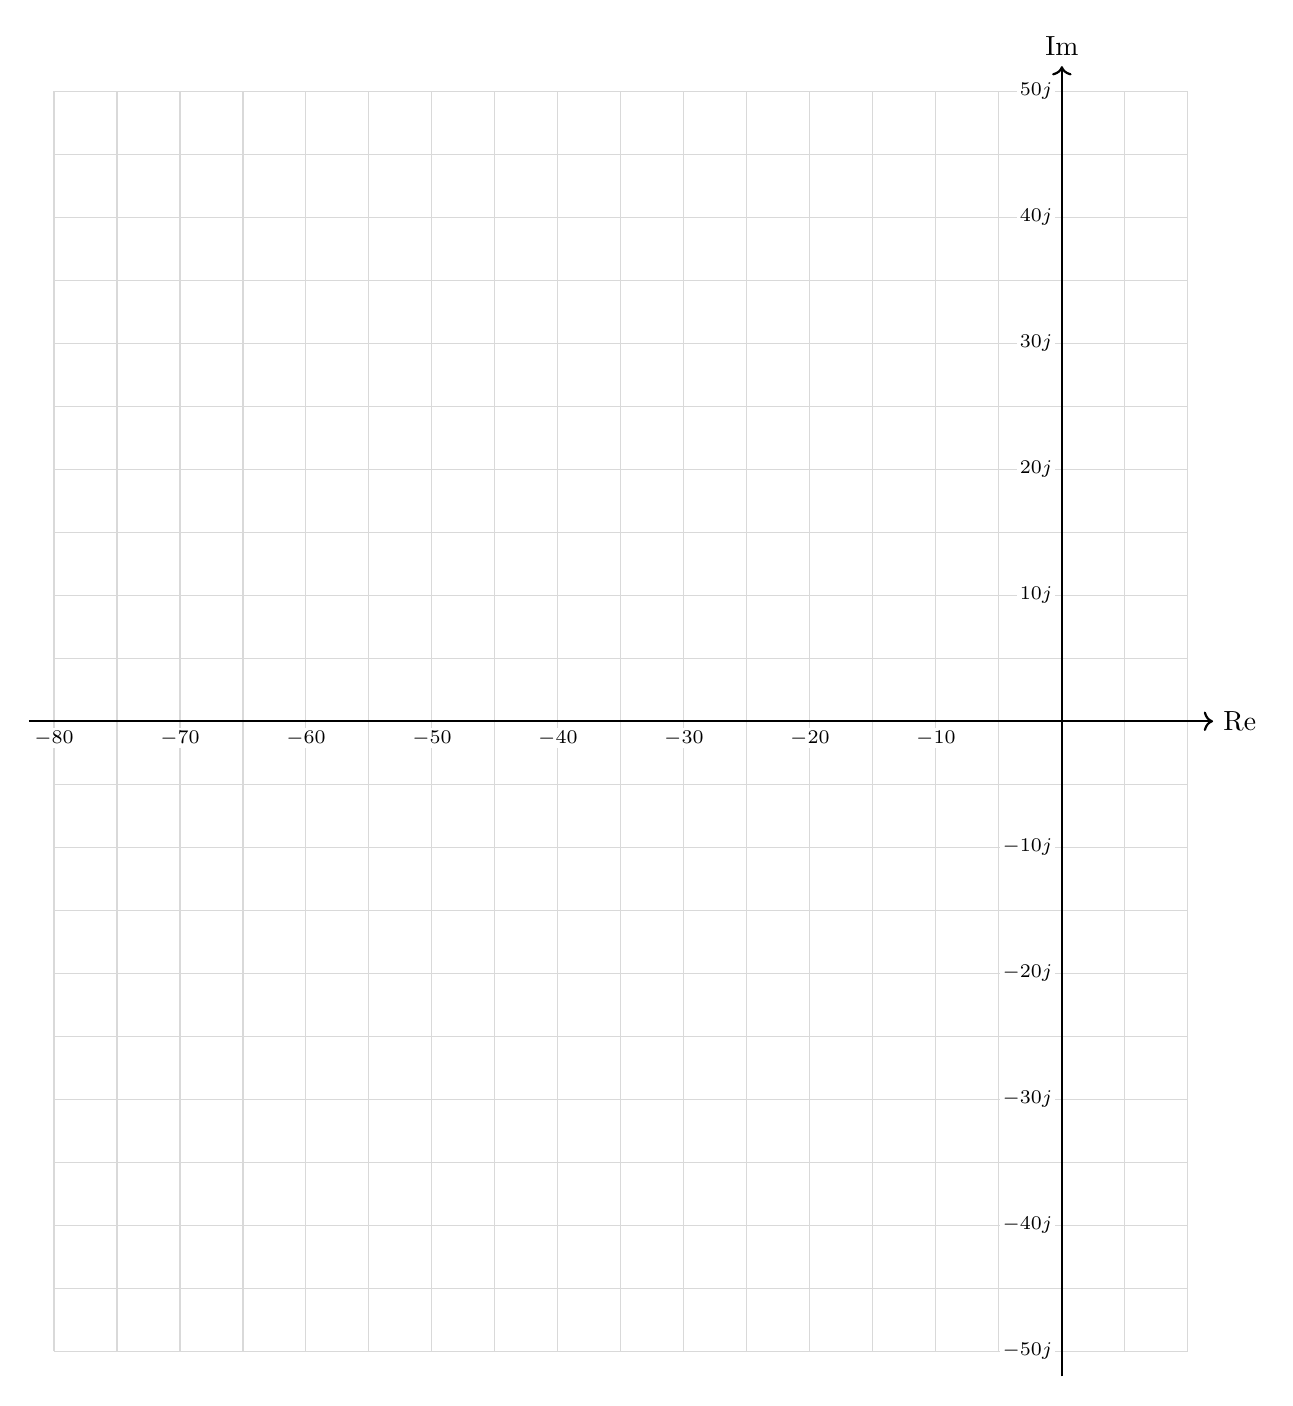
\begin{tikzpicture}[x=0.16cm, y=0.16cm]
    \draw[gray!30, thin, step=5] (-80,-50) grid (10,50);
    \draw[->, thick] (-82,0) -- (12,0) node[right] {$\mathrm{Re}$};
    \draw[->, thick] (0,-52) -- (0,52) node[above] {$\mathrm{Im}$};
    \foreach \x in {-80,-70,...,-10}
      \node[below, font=\scriptsize, fill=white, inner sep=1pt] at (\x,-0.5) {$\x$};
    \foreach \y in {-50,-40,...,-10,10,20,...,50}
      \node[left, font=\scriptsize, fill=white, inner sep=1pt] at (-0.5,\y) {$\y j$};
  \end{tikzpicture}
  \caption{Region of acceptable closed-loop poles for $t_s \le 0.1$ s and $M_p \le 5\%$.}
\end{figure}

\clearpage
\problem{4.29(d)}{PD Controller}
\prompt{Give values for $k_p$ and $k_d$ for a PD controller, $u(t) = k_d\dot e(t) + k_p e(t)$, which meets the specifications. For hand tuning write it as $G_c(s) = K_c(\tau_c s + 1)$, with $k_d = K_c\tau_c$ and $k_p = K_c$.}

\subpart{4.29(d).i}
\prompt{Symbolically form $T_{de}(s)$. What is the expression for the disturbance steady-state error (the DC gain of $T_{de}(s)$)? What are the requirements on $K_c$ and $\tau_c$ to meet the disturbance-SSE requirement?}
\answer{}

\subpart{4.29(d).ii}
\prompt{Explore the root locus for various $\tau_c$. Find $\tau_c$ for which the branches pass into the region from part (c), and an initial $K_c$ that places the closed-loop poles there while also meeting the minimum $K_c$ for the disturbance SSE.}
\answer{}

\subpart{4.29(d).iii}
\prompt{Form $T_{ry}(s)$ and examine the step response. Iteratively adjust the design (mainly $\tau_c$) to meet: SSE $\le 0.01$ rad/s, $t_s \le 0.1$ s, $M_p \le 10\%$.}
\answer{}

\subpart{4.29(d).iv}
\prompt{Verify the design: $T_{de}$ for the steady-state error requirement, and the step response of $T_{ry}$ for settling time and overshoot.}
\answer{}

\clearpage
\problem{4.29(e)}{Eliminating the Disturbance Error}
\prompt{Plot the step response of $T_{de}(s)$. Does the PD controller from part (d) meet the requirement? How would the disturbance-induced steady-state error change with this controller, and what controller structure would make it zero?}
\answer{}

\problem{Extra Credit}{}
\prompt{Engineer a controller that meets the $t_s$ and $M_p$ requirements with zero disturbance steady-state error.}
\answer{}


\end{document}
